\documentclass[border=10pt]{standalone}
\usepackage[T1]{fontenc}
\usepackage{helvet}
\renewcommand{\familydefault}{\sfdefault}
\usepackage{tikz}
\usetikzlibrary{arrows.meta,positioning,calc,decorations.pathreplacing,fit}

\definecolor{idpblue}{HTML}{005DAA}
\definecolor{idpcyan}{HTML}{00B3FF}
\definecolor{warm}{HTML}{D7263D}
\definecolor{inkgray}{HTML}{444444}
\definecolor{forestgreen}{HTML}{2E7D32}

\begin{document}
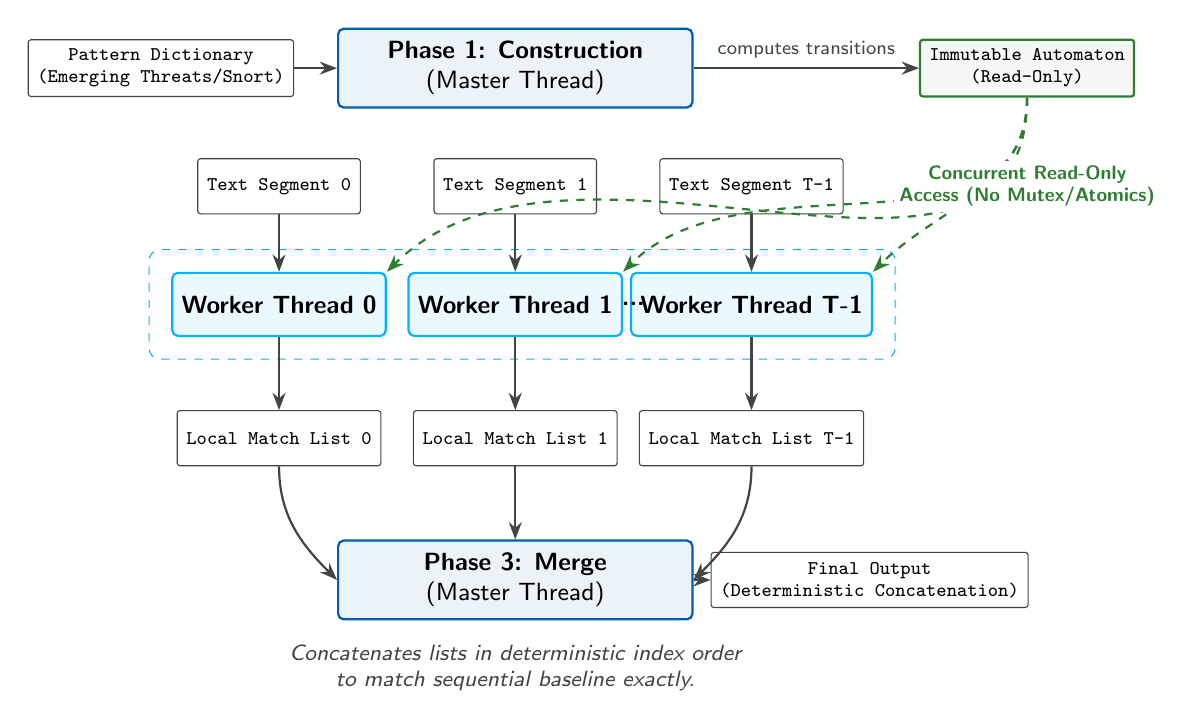
\begin{tikzpicture}[
    font=\small,
    >={Stealth[length=2.2mm]},
    phase/.style={draw=inkgray, fill=gray!5, thick, rounded corners=2pt, minimum width=45mm, minimum height=10mm, align=center},
    seqphase/.style={phase, draw=idpblue, fill=idpblue!8},
    parphase/.style={phase, draw=idpcyan, fill=idpcyan!8},
    data/.style={draw=inkgray, fill=white, rounded corners=1pt, minimum width=25mm, minimum height=7mm, align=center, font=\scriptsize\ttfamily},
    shared/.style={data, draw=forestgreen, fill=forestgreen!5, thick},
    arrow/.style={inkgray, ->, line width=0.8pt},
    readarrow/.style={forestgreen, ->, line width=0.8pt, dashed},
    label/.style={font=\bfseries},
    caption/.style={font=\footnotesize\itshape, text=inkgray, align=center},
]

    % =====================================================================
    % PHASE 1: CONSTRUCTION (Sequential)
    % =====================================================================
    \node[seqphase] (p1) at (0, 4.5) {\textbf{Phase 1: Construction}\\\small(Master Thread)};
    \node[data] (in_dict) at (-4.5, 4.5) {Pattern Dictionary\\(Emerging Threats/Snort)};
    \node[shared] (shared_auto) at (6.5, 4.5) {Immutable Automaton\\(Read-Only)};

    \draw[arrow] (in_dict) -- (p1);
    \draw[arrow] (p1) -- (shared_auto) node[midway, above, font=\scriptsize] {computes transitions};

    % =====================================================================
    % PHASE 2: SEARCH (Parallel)
    % =====================================================================
    % Parallel threads
    \node[parphase, minimum width=25mm, minimum height=8mm] (t0) at (-3.0, 1.5) {\textbf{Worker Thread 0}};
    \node[parphase, minimum width=25mm, minimum height=8mm] (t1) at (0, 1.5) {\textbf{Worker Thread 1}};
    \node[parphase, minimum width=25mm, minimum height=8mm] (tN) at (3.0, 1.5) {\textbf{Worker Thread T-1}};
    \node at (1.5, 1.5) {\textbf{...}};

    % Fit a boundary box for parallel search
    \node[draw=idpcyan, dashed, inner sep=8pt, rounded corners=4pt, label={[idpcyan, font=\bfseries]above:Phase 2: Search (Parallel \& Lock-Free)}] (fit_p2) [fit=(t0) (t1) (tN)] {};

    % Thread inputs (text chunks)
    \node[data, minimum width=20mm] (txt0) at (-3.0, 3.0) {Text Segment 0};
    \node[data, minimum width=20mm] (txt1) at (0, 3.0) {Text Segment 1};
    \node[data, minimum width=20mm] (txtN) at (3.0, 3.0) {Text Segment T-1};

    \draw[arrow] (txt0) -- (t0);
    \draw[arrow] (txt1) -- (t1);
    \draw[arrow] (txtN) -- (tN);

    % Read transitions from shared automaton (lock-free!)
    \draw[readarrow] (shared_auto.south) to[out=-90, in=45] (tN.north east);
    \draw[readarrow] (shared_auto.south) to[out=-90, in=45] (t1.north east);
    \draw[readarrow] (shared_auto.south) to[out=-90, in=45] (t0.north east);
    \node[forestgreen, font=\scriptsize\bfseries, align=center, anchor=west, fill=white, inner sep=2pt] at (4.8, 3.0) {Concurrent Read-Only\\Access (No Mutex/Atomics)};

    % Thread outputs (local match lists)
    \node[data, minimum width=20mm] (list0) at (-3.0, -0.2) {Local Match List 0};
    \node[data, minimum width=20mm] (list1) at (0, -0.2) {Local Match List 1};
    \node[data, minimum width=20mm] (listN) at (3.0, -0.2) {Local Match List T-1};

    \draw[arrow] (t0) -- (list0);
    \draw[arrow] (t1) -- (list1);
    \draw[arrow] (tN) -- (listN);

    % =====================================================================
    % PHASE 3: MERGE (Sequential)
    % =====================================================================
    \node[seqphase] (p3) at (0, -2.0) {\textbf{Phase 3: Merge}\\\small(Master Thread)};
    \node[data] (out_matches) at (4.5, -2.0) {Final Output\\(Deterministic Concatenation)};

    \draw[arrow] (list0.south) to[out=-90, in=135] (p3.west);
    \draw[arrow] (list1.south) -- (p3.north);
    \draw[arrow] (listN.south) to[out=-90, in=45] (p3.east);

    \draw[arrow] (p3) -- (out_matches);

    % Labels/captures
    \node[caption, anchor=north] at (0, -2.7) {Concatenates lists in deterministic index order\\to match sequential baseline exactly.};

\end{tikzpicture}
\end{document}
